\documentclass[aps,pra,showpacs,notitlepage,onecolumn,superscriptaddress,nofootinbib]{revtex4-1}
\usepackage[utf8]{inputenc}
\usepackage[tmargin=1in, bmargin=1.25in, lmargin=1.5in, rmargin=1.5in]{geometry}
\usepackage{amsmath, amssymb, amsthm}
\usepackage{graphicx}
\usepackage{xcolor}
\usepackage{enumitem}
\usepackage{datetime}
\usepackage{hyperref}
\usepackage{titlesec}
\usepackage{import}
\usepackage{mathtools}
\usepackage{thmtools,thm-restate}
\usepackage{tikz-cd}


% package for commutative diagrams
% \usepackage{tikz-cd}

%%%%%%%%%%%%%%%%%%%%%%%%%%%%%%%%%%%%%%%%%%%%%
\definecolor{crimson}{RGB}{186,0,44}
\definecolor{moss}{RGB}{0, 186, 111}
\newcommand{\pop}[1]{\textcolor{crimson}{#1}}
\newcommand{\zcom}[1]{\noindent\textcolor{crimson}{(Z): #1}}
\newcommand{\jcom}[1]{\noindent\textcolor{moss}{(J): #1}}
\newcommand{\wt}[1]{\widetilde{#1}}
\newcommand{\pqeq}{\succcurlyeq}
\newcommand{\pleq}{\preccurlyeq}
\newcommand{\Wedge}{\bigwedge}

%%%%%%%%%%%%%%%%%%%%%%%%%%%%%%%%%%%%%%%%%%%%%
\hypersetup{
    colorlinks,
    linkcolor={crimson},
    citecolor={crimson},
    urlcolor={crimson}
}

\usepackage{qcircuit}

%%%%%%%%%%%%%%%%%%%%%%%%%%%%%%%%%%%%%%%%%%%%%
\theoremstyle{definition}
\newtheorem{definition}{Definition}[section]
\newtheorem{lemma}{Lemma}[section]
\newtheorem{theorem}{Theorem}[section]
\newtheorem{corollary}{Corollary}[theorem]
\newtheorem*{theorem*}{Theorem}
\newtheorem*{corollary*}{Corollary}
\newtheorem{remark}{Remark}[section]
\newtheorem{conjecture}{Conjecture}[section]
\newtheorem{example}{Example}[section]
\newtheorem{reminder}{Reminder}[section]
\newtheorem{problem}{Problem}[section]
\newtheorem{question}{Question}[section]
\newtheorem{answer}{Answer}[section]
\newtheorem{fact}{Fact}[section]
\newtheorem{claim}{Claim}[section]

\newcommand{\hhrulefill}{\hspace{-1.5em} \hrulefill}

\usepackage{geometry}
\geometry{
  left=25mm,
  right=25mm,
  top=20mm,
}

%%%%%%%%%%%%%%%%%%%%%%%%%%%%%%%%%%%%%%%%%%%%%
\bibliographystyle{unsrt}

%%%%%%%%%%%%%%%%%%%%%%%%%%%%%%%%%%%%%%%%%%%%%
%%%%%%%%%%%%%%%%%%%%%%%%%%%%%%%%%%%%%%%%%%%%%
%%%%%%%%%%%%%%%%%%%%%%%%%%%%%%%%%%%%%%%%%%%%%

\begin{document}

\title{Discrete Riemann geometry and the Ising model}
\author{Jack Ceroni}
\email{jackceroni@gmail.com}

\date{\today}

\maketitle

\section{Introduction}

\noindent The goal of these lecture notes is to exposit, in detail, some of the fundamental constructions in Mercat's formulation of discrete Riemannian geometry.
Our notes begin with the assumption that the reader is already familiar with the first half of Section 2.1 of Mercat's paper \emph{Discrete Riemann surfaces and the Ising model},
up until the explanation of discrete de Rham complexes.

\section{Discrete de Rham homology and cohomology}

\noindent In the first part of Section 2.1, Mercat gives the discrete structure on which discrete analogues of differential-geometric
constructs are defined, the so-called cellular decomposition $\Gamma$, it dual $\Gamma^{*}$, and their natural pairing, the \emph{double} $\Lambda$.

\begin{center}
  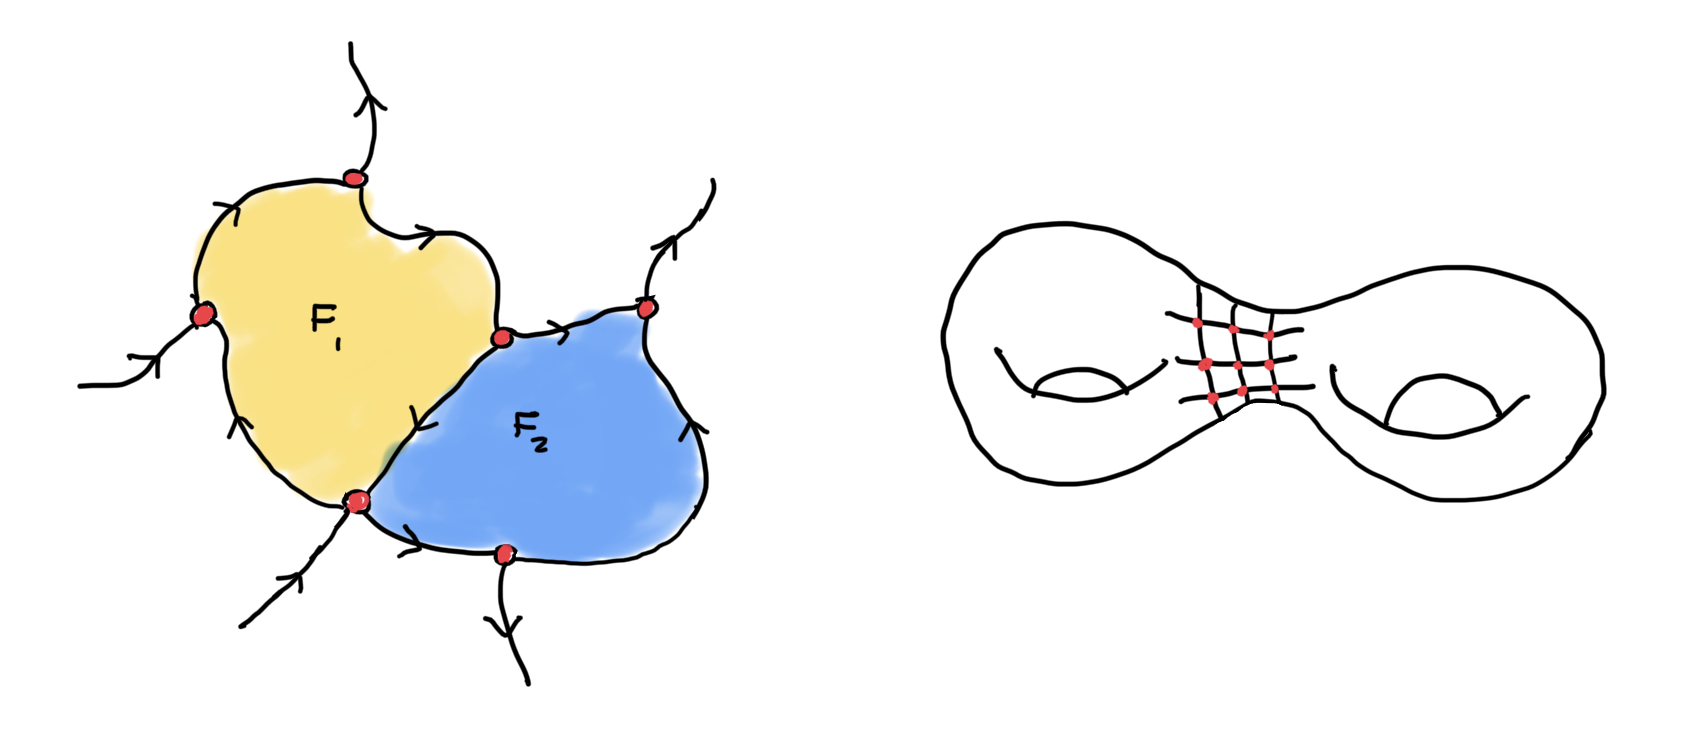
\includegraphics[width=\textwidth]{./assets/mercat1.jpeg}
\end{center}

\noindent Mercat
then defines the notion of a chain on the discrete structure, and a corresponding boundary operation. With a boundary operator defined,
a natural next step is to consider the corresponding \emph{singular homology} and \emph{singular cohomology}. In particular, the singular homology
is derived from chain complex:
% https://q.uiver.app/#q=WzAsMyxbMCwwLCJDX2soXFxMYW1iZGEpIl0sWzEsMCwiQ18xKFxcTGFtYmRhKSJdLFsyLDAsIkNfezJ9KFxcTGFtYmRhKSJdLFsyLDEsIlxccGFydGlhbCIsMl0sWzEsMCwiXFxwYXJ0aWFsIiwyXV0=
\[\begin{tikzcd}
	          {C_0(\Lambda)} & {C_1(\Lambda)} & {C_{2}(\Lambda)}
	          \arrow["\partial"', from=1-3, to=1-2]
	          \arrow["\partial"', from=1-2, to=1-1]
\end{tikzcd}\]
and the corresponding singular cohomology is given by taking the dual, yielding the cochain complex
% https://q.uiver.app/#q=WzAsMyxbMCwwLCJcXHRleHR7SG9tfShDXzAoXFxMYW1iZGEpLCBcXG1hdGhiYntDfSkiXSxbMSwwLCJcXHRleHR7SG9tfShDXzEoXFxMYW1iZGEpLCBcXG1hdGhiYntDfSkiXSxbMiwwLCJcXHRleHR7SG9tfShDXzIoXFxMYW1iZGEpLCBcXG1hdGhiYntDfSkiXSxbMSwyLCJcXHBhcnRpYWxeeyp9Il0sWzAsMSwiXFxwYXJ0aWFsXnsqfSJdXQ==
\[\begin{tikzcd}
	          {\text{Hom}(C_0(\Lambda), \mathbb{C})} & {\text{Hom}(C_1(\Lambda), \mathbb{C})} & {\text{Hom}(C_2(\Lambda), \mathbb{C})}
	          \arrow["{\partial^{*}}", from=1-2, to=1-3]
	          \arrow["{\partial^{*}}", from=1-1, to=1-2]
\end{tikzcd}\]
where we will define $d \coloneqq \partial^{*}$ as the dual of the boundary operation (the coboundary) acting on the dual spaces $C^{k}(\Lambda) \coloneqq \text{Hom}(C_k(\Lambda), \mathbb{C})$ (spaces of $k$-cochains).

\begin{remark}[Standard de Rham cohomology]
  Given a manifold $M$, the \emph{de Rham cohomology} is given by the complex of differential $k$-forms on $M$, connected by the exterior derivative $d : \Omega^{k}(M) \rightarrow \Omega^{k + 1}(M)$:
  % https://q.uiver.app/#q=WzAsNSxbMCwwLCJcXGNkb3RzIl0sWzEsMCwiXFxPbWVnYV57ayAtIDF9KE0pIl0sWzIsMCwiXFxPbWVnYV57a30oTSkiXSxbMywwLCJcXE9tZWdhXntrICsgMX0oTSkiXSxbNCwwLCJcXGNkb3RzIl0sWzAsMSwiZCJdLFsxLDIsImQiXSxbMiwzLCJkIl0sWzMsNCwiZCJdXQ==
  \[\begin{tikzcd}
  \cdots & {\Omega^{k - 1}(M)} & {\Omega^{k}(M)} & {\Omega^{k + 1}(M)} & \cdots
  \arrow["d", from=1-1, to=1-2]
  \arrow["d", from=1-2, to=1-3]
  \arrow["d", from=1-3, to=1-4]
  \arrow["d", from=1-4, to=1-5]
  \end{tikzcd}\]
  Similar to above, the singular cohomology is derived from the complex of $k$-cochains:
  % https://q.uiver.app/#q=WzAsNSxbMCwwLCJcXGNkb3RzIl0sWzEsMCwiXFx0ZXh0e0hvbX0oQ157ayAtIDF9KE0pKSJdLFsyLDAsIlxcdGV4dHtIb219KENee2t9KE0pKSJdLFszLDAsIlxcdGV4dHtIb219KENee2sgKyAxfShNKSkiXSxbNCwwLCJcXGNkb3RzIl0sWzAsMSwiXFxwYXJ0aWFsXnsqfSJdLFsxLDIsIlxccGFydGlhbF57Kn0iXSxbMiwzLCJcXHBhcnRpYWxeeyp9Il0sWzMsNCwiXFxwYXJ0aWFsXnsqfSJdXQ==
  \[\begin{tikzcd}
  \cdots & {\text{Hom}(C^{k - 1}(M))} & {\text{Hom}(C^{k}(M))} & {\text{Hom}(C^{k + 1}(M))} & \cdots
  \arrow["{\partial^{*}}", from=1-1, to=1-2]
  \arrow["{\partial^{*}}", from=1-2, to=1-3]
  \arrow["{\partial^{*}}", from=1-3, to=1-4]
  \arrow["{\partial^{*}}", from=1-4, to=1-5]
  \end{tikzcd}\]
  There is a fundamental result in differential geometry called \emph{de Rham's theorem}, which states that the $k$-th de Rham cohomology group is
  isomorphic to the $k$-th singular cohomology group. It is for this reason that we can take the approach of considering the discrete singular cohomology,
  and recover objects which resemble those associated with the de Rham cohomology, like the exterior derivative, the Hodge star (as we will see), and more.
  This is also the reason for notational choices such as $d \coloneqq \partial^{*}$, as well as:
  \begin{equation}
    \omega(s) \coloneqq \displaystyle\int_{s} \omega \ \ \ \ \text{with} \ \ \ \ \omega \in C^{k}(\Lambda), \ s \in C_k(\Lambda).
  \end{equation}
  In particular, evaluating cochains is ``equivalent'' in a sense, via the de Rham isomorphism, to integrating forms.
\end{remark}

\noindent From the definition of $d \coloneqq \partial^{*}$, Stokes' theorem becomes a tautology:
\begin{equation}
  \displaystyle\int_{s} d\omega = \partial^{*}(\omega)(s) = \omega(\partial s) = \displaystyle\int_{\partial s} \omega.
\end{equation}

\section{Discrete Hodge star}

\noindent The next differential-geometric construct we will attempt to translate to the discrete picture is the \emph{Hodge star}.

\begin{definition}[The standard Hodge star]
  At a high-level, the Hodge star can be thought of as an operation which, given a differential form $\omega$, ``completes it'' so that the wedge of $\omega$
  and its starred counterpart is the volume form on the manifold.

  Let us be more specific. Suppose $(M, g_p)$ is an oriented, smooth, $n$-dimensional pseudo-Riemannian manifold. The metric $g_p$ induces a natural
  isomorphism $\Phi$ between $T_p M$ and $T_p^{*} M$, where tangent vector $v_p$ is mapped to $g_p(v, \cdot)$. We also know that the space of alternating $k$-tensors on $T_p M$
  is precisely the $k$-fold wedge of $T_p^{*} M$, denoted $\Wedge^{k} T_p^{*} M$. From here, we have a canonical bilinear form $\langle\cdot, \cdot\rangle$ on $\Omega^{k}(M)$ to $\Omega^{0}(M)$, namely
  \begin{equation}
    \langle \alpha_1(p) \wedge \cdots \wedge \alpha_k(p), \beta_1(p) \wedge \cdots \wedge \beta_k(p) \rangle \coloneqq \det \left( \left[ g_p(\Phi^{-1}(\alpha_i(p)), \Phi^{-1}(\beta_j(p))) \right]_{i, j = 1}^{k} \right).
  \end{equation}
  $M$ also comes equipped with a volume form $\text{vol}$ induced by $g_p$. The \emph{Hodge star} is defined to be the unique linear map $* : \Omega^{k}(M) \rightarrow \Omega^{n - k}(M)$
  such that
  \begin{equation}
    \alpha \wedge * \beta = \langle \alpha, \beta \rangle \text{vol}
    \end{equation}
  Of course, existence and uniqueness of this operator must be proved (we will omit these proofs, but they are standard in differential geometry literature). Note that in particular, we have
  $\alpha \wedge * \alpha = \text{vol}$ for any form $\alpha$. Also note that we can define a different Hodge star for each $\Omega^{k}(M)$, with $0 \leq k \leq n$.
\end{definition}

\begin{example}[The Hodge star on a surface]
  For the case of a surface, the family of Hodge stars we can define are mappings $* : \Omega^{0}(M) \rightarrow \Omega^{2}(M)$, $* : \Omega^{1}(M) \rightarrow \Omega^{1}(M)$, and $* : \Omega^{2}(M) \rightarrow \Omega^{0}(M)$.
  One can verify that, in this case,
  \begin{align}
    * 1 = \sqrt{\det g } \ dx \wedge dy \ \ \ \ \ \ \ \ \ \ \ * (dx \wedge dy) = \frac{1}{\sqrt{\det g }} \\
    * dx =  \sqrt{\det g } \left( g^{11} dy - g^{12} dx \right) \ \ \ \ \ \ * dy = \sqrt{\det g } \left( g^{21} dy - g^{22} dx \right)
  \end{align}
  where $g \coloneqq [g_{ij}]$ is the matrix of components of the metric tensor in the standard basis, and $[g^{ij}]$ is the corresponding inverse. Under the assumption that the metric is diagonal, we have
  $\det g = g_{11} g_{22}$. Making this assumption, and integrating over regions, we find
  \begin{align}
    \label{eq:form2}
    \displaystyle\int_{\Omega} * f = \displaystyle\int_{\Omega} \sqrt{\det g} \ f dx \wedge dy \ \ \ \ \ \ \displaystyle\int_{x} * \left( \sqrt{\det g} \ f dx \wedge dy \right) = f(x)
  \end{align}
  as well as
  \begin{align}
    \label{eq:form}
    \displaystyle\int_{\gamma} * \sqrt{g_{11}} dx = \displaystyle\int_{\gamma} \sqrt{ g_{22}} dy \ \ \ \ \ \displaystyle\int_{\gamma} * \sqrt{g_{22}} dy = - \displaystyle\int_{\gamma} \sqrt{ g_{11}} dx.
  \end{align}
\end{example}

\noindent This example serves to motivate our definition of the \emph{discrete Hodge star}. If we think about vertices/edges/faces as being the fundamental, ``infinitesimal'' objects in our discrete theory,
it makes sense to think of integrals over curves/regions in the discrete picture as being sums over edges/faces. In the standard picture, this infinitesimal area is associated with the area element $dA = \sqrt{\det g} \ dx \wedge dy$.
Similarly, we have length elements in the $x$ and $y$ directions $\sqrt{g_{11}} dx$ and $\sqrt{g_{22}} dy$ respectively.

Via Eq.~\eqref{eq:form2}, when we integrate $* f$ over an area, we are effectively just averaging $f$ on the region. In our \emph{discrete} picture, we associate this operation to evaluating a function $f \in C^0(\Lambda)$
on the \emph{dual face}. Similarly, when we evaluate a the Hodge star of a $2$-form $* (\sqrt{\det g} \ f dx \wedge dy)$ at a point, we can think of this as evaluating the $2$-form on a point which ``encodes'' the average value
over the face. In our discrete picture, we take this point to be precisely the \emph{dual point} of a face. Thus, for $f \in C^{0}(\Lambda)$ and $\omega \in C^{2}(\Lambda)$, we define
\begin{equation}
  \int_{F} * f \coloneqq f(F^{*}) \ \ \ \ \ \text{and} \ \ \ \ \ \int_{x} * \omega \coloneqq \omega(* x)
\end{equation}

\hhrulefill

\begin{remark}
  \label{rem:a}
In a similar fashion, if we think of a discrete curve as a discretized sum over infinitesimal edges ($x$-direction length elements) and dual edges ($y$-direction length elements),
the integral over a form $\sqrt{g_{11}} dx$ will effectively ``pick out'' all the $x$-direction elements and multiply by an associated length. Similarly,
$\sqrt{g_{22}} dy$ will effectively ``pick out'' all the $y$-direction elements and multiply by an associated length. The Hodge star interchanges these forms, in a sense.
\end{remark}

\hhrulefill

\noindent To be more specific, in the discrete picture, suppose $\alpha \in C^{1}(\Gamma)$, so that $\alpha$ is only non-zero on ``$x$-direction length elements'' (the same exact reasoning
applies to the case of $\alpha \in C^{1}(\Gamma^{*})$). Then, $\alpha$ evaluated on a ``curve'',
\begin{equation}
  \gamma = \gamma_1 + \gamma_2 = (a_1 e_1 + \cdots + a_j e_j) + (b_1 e^{*}_1 + \cdots + b_j e_j^{*})
\end{equation}
with $e_j$ edges and $e_j^{*}$ dual edges is simply given by $\int_{\gamma} \alpha = \int_{\gamma_1} \alpha = \sum_{i} a_i \int_{e_i} \alpha$: the integral ``picks out'' the $x$-direction components
of the curve. Taking the dual, $\gamma^{*}$, the corresponding integral will ``pick out'' the $y$-direction components, $\int_{\gamma^{*}} \alpha = \int_{\gamma_2} \alpha = \sum_{i} b_i \int_{e_i} \alpha$.
It follows from this fact, and the logic of Rem.~\ref{rem:a}, that the discrete Hodge star should effectively dualize the edge on which a form is being evaluated, and modify the length interval utilized to perform the integral.

Making the canonical substitution of the metric elements for the discrete edge-lengths, $g_{11} \mapsto \ell(e)^2$ and $g_{22} \mapsto \ell(e^{*})^2$, we define
\begin{equation}
  \displaystyle\int_{e} * \alpha \coloneqq - \sqrt{\frac{\ell(e^{*})^2}{\ell(e)^2}} \displaystyle\int_{e^{*}} \alpha = - \rho(e^{*}) \displaystyle\int_{e^{*}} \alpha
  \end{equation}

\noindent With this definition, we can make note of some basic facts about the discrete Hodge star, which are direct translations of results from standard differential geometry.

\begin{remark}
  For the sake of notational clarity, let $*_{k} : C^{k}(\Lambda) \rightarrow C^{2 - k}(\Lambda)$. Then it is easy to check that $*_{k} \circ *_{n - k} = (-1)^{k (n - k)}$. In particular,
  $*_0 \circ *_{2} = *_{2} \circ *_0 = 1$, so $C^{0}(\Lambda)$ and $C^{2}(\Lambda)$ are isomorphic as modules, via the Hodge star.
\end{remark}

\begin{remark}[Holomorphic forms]
  \label{rem:b}
  It is easy exercise to check that a function $f$ is \emph{discrete holomorphic}, with respect to the definition provided in the first part of Section 2.1 if and only if $* df = -i df$.
  Moreover, we say that a $1$-form $\alpha$ is discrete holomorphic if and only if it is closed, $d\alpha = 0$, and satisfies $* \alpha = -i \alpha$ (this is precisely how holomorphic forms
  are defined in the standard differential-geometric picture as well).
  \end{remark}

\section{Discrete Dolbeault complex}

\noindent Consider the Hodge star $* : C^{1}(\Lambda) \rightarrow C^{1}(\Lambda)$. We know that $*^2 = -1$, implying $(* + i) (* - i) = 0$. Note that $*$ is a linear operator,
so this implies that its eigenvalues must be contained in the set $\{ \pm i \}$.

\begin{lemma}
We can decompose $C^{1}(\Lambda)$ into a direct sum of its respective eigenspaces, $C^{1}(\Lambda) = C^{(1, 0)}(\Lambda) \oplus C^{(0, 1)}(\Lambda)$, with projections
\begin{equation}
  \pi_{(1, 0)} = \frac{1}{2} ( 1 + i *) \ \ \ \ \text{and} \ \ \ \ \pi_{(0, 1)} = \frac{1}{2} (1 - i *).
\end{equation}
\end{lemma}
\begin{proof}
  Let $v \in C^{1}(\Lambda)$. Clearly, $v = \pi_{(1, 0)} v + \pi_{(0, 1)} v$. We have
  \begin{equation}
    * \left( \frac{1}{2} (1 \pm i *) v \right) = \frac{1}{2} (\mp i + *) v = \mp i \left( \frac{1}{2} (1 \pm i *) \right) v
  \end{equation}
  so $\pi_{(1, 0)} v$ and $\pi_{(0, 1)} v$ are in the desired eigenspaces. Of course, the resulting sum of subspaces is direct, as any vector $v \in C^{1}(\Lambda)$ with $v \neq 0$ cannot be both a $i$ and a $-i$-eigenvector.
  \end{proof}

\noindent Note that from Rem.~\ref{rem:b}, we can equivalently say that a $1$-form is discrete holomorphic if and only if it is closed and in the $(1, 0)$-eigenspace of $C^{1}(\Lambda)$.
Similarly, we say that a $1$-form is \emph{discrete antiholomorphic} if and only if it is closed and in the $(0, 1)$-eigenspace.

The decomposition of the de Rham complex into holomorphic and antiholomorphic parts is what leads to the \emph{Dolbeault complex} in standard differential geometry. We have
an analogous construction here. For notational clarity, let $d_k : C^{k}(\Lambda) \rightarrow C^{k + 1}(\Lambda)$. We define $d'_0 = \pi_{(1, 0)} \circ d_0$ and $d''_0 = \pi_{(0, 1)} \circ d_0$ as the projections of the coboundary
onto the holomorphic and antiholomorphic components. Moreover, we define $d'_1 = d_1 \circ \pi_{(1, 0)}$ and $d''_1 = d_1 \circ \pi_{(0, 1)}$ as the coboundary of the projections onto holomorphic and
antiholomorphic components. It follows from the definitions that
\begin{equation}
  d_1 \circ d_0 = 0 \ \ \ \ \Longrightarrow \ \ \ \ d_1' \circ d_0' = 0 \ \ \ \ \text{and} \ \ \ \ d_1'' \circ d_0'' = 0.
\end{equation}
and, in direct analogy to the standard Dolbeault structure, we have the following complex:
% https://q.uiver.app/#q=WzAsNCxbMSwyLCJDXjAoXFxMYW1iZGEpIl0sWzAsMSwiQ157KDEsIDApfShcXExhbWJkYSkiXSxbMiwxLCJDXnsoMCwgMSl9KFxcTGFtYmRhKSJdLFsxLDAsIkNeMihcXExhbWJkYSkiXSxbMCwxLCJkXzAnIl0sWzAsMiwiZF8wJyciLDJdLFsxLDMsImRfMSciXSxbMiwzLCJkXzEnJyIsMl1d
\[\begin{tikzcd}
& {C^2(\Lambda)} \\
	          {C^{(1, 0)}(\Lambda)} && {C^{(0, 1)}(\Lambda)} \\
	          & {C^0(\Lambda)}
	          \arrow["{d_0'}", from=3-2, to=2-1]
	          \arrow["{d_0''}"', from=3-2, to=2-3]
	          \arrow["{d_1'}", from=2-1, to=1-2]
	          \arrow["{d_1''}"', from=2-3, to=1-2]
\end{tikzcd}\]

\section{Discrete Laplacian}

\noindent It may not come as a large surprise after defining the discrete Hodge star that it is also possible to define a discrete analogue of the Laplacian.
It is a fact that in the standard differential-geometric picture, we can write the Laplacian as
\begin{equation}
  \label{eq:lap}
  \Delta \coloneqq -d * d * - * d * d
\end{equation}
for the standard exterior derivative and Hodge star. We take this formula as the \emph{definition} of the discrete Laplacian in the discrete picture, where $*$ is the discrete Hodge star and $d$ is the coboundary.

\begin{lemma}
  For a function $f \in C^{0}(\Lambda)$, the definition of the Laplacian given in Eq.~\eqref{eq:lap} is equivalent to the standard, graph-theoretic definition of the Laplacian for a function
  on the nodes of a graph,
  \begin{equation}
    (\Delta f)(x) = \displaystyle\sum_{y \in n(x)} \rho((x, y)) (f(x) - f(y))
  \end{equation}
  where $n(x)$ is the set of neighbours of node $x$ in graph $\Gamma$.
\end{lemma}

\begin{proof}
  This is a straightforward application of the definitions of each operation. Note that $* f \in C^{2}(\Lambda)$, so $d(* f) = 0$. Thus,
  in this case, $-d * d * - * d * d = - * d * d$. We then have
  \begin{align}
    -(* d * d)(f)(x) &= - \displaystyle\int_{x^{*}} (d * d)(f) = -\displaystyle\int_{\partial x^{*}} (* d)(f) = - \displaystyle\sum_{y \in n(x)} \displaystyle\int_{(x, y)^{*}} (* d)(f)
    \\ & = \displaystyle\sum_{y \in n(x)} \rho(-(x, y)) \displaystyle\int_{-(x, y)} df = \displaystyle\sum_{y \in n(x)} \rho((x, y)) \displaystyle\int_{(y, x)} df = \displaystyle\sum_{y \in n(x)} \rho((x, y)) (f(x) - f(y))
  \end{align}
  where we know that $(e^{*})^{*} = -e$ and $\rho(-e) = \rho(e)$.

\end{proof}

\noindent This proof can be depicted visually, where each step demonstrates at a corse-grained level exactly which portions of the dual $\Lambda$ are ``selected'' by each of the operations making up the discrete Laplacian.
As can be seen, at the final stage, we have arrived at a sum over the node $x$, highlighted in red through all the diagrams, as well as its neighbours:
\begin{center}
  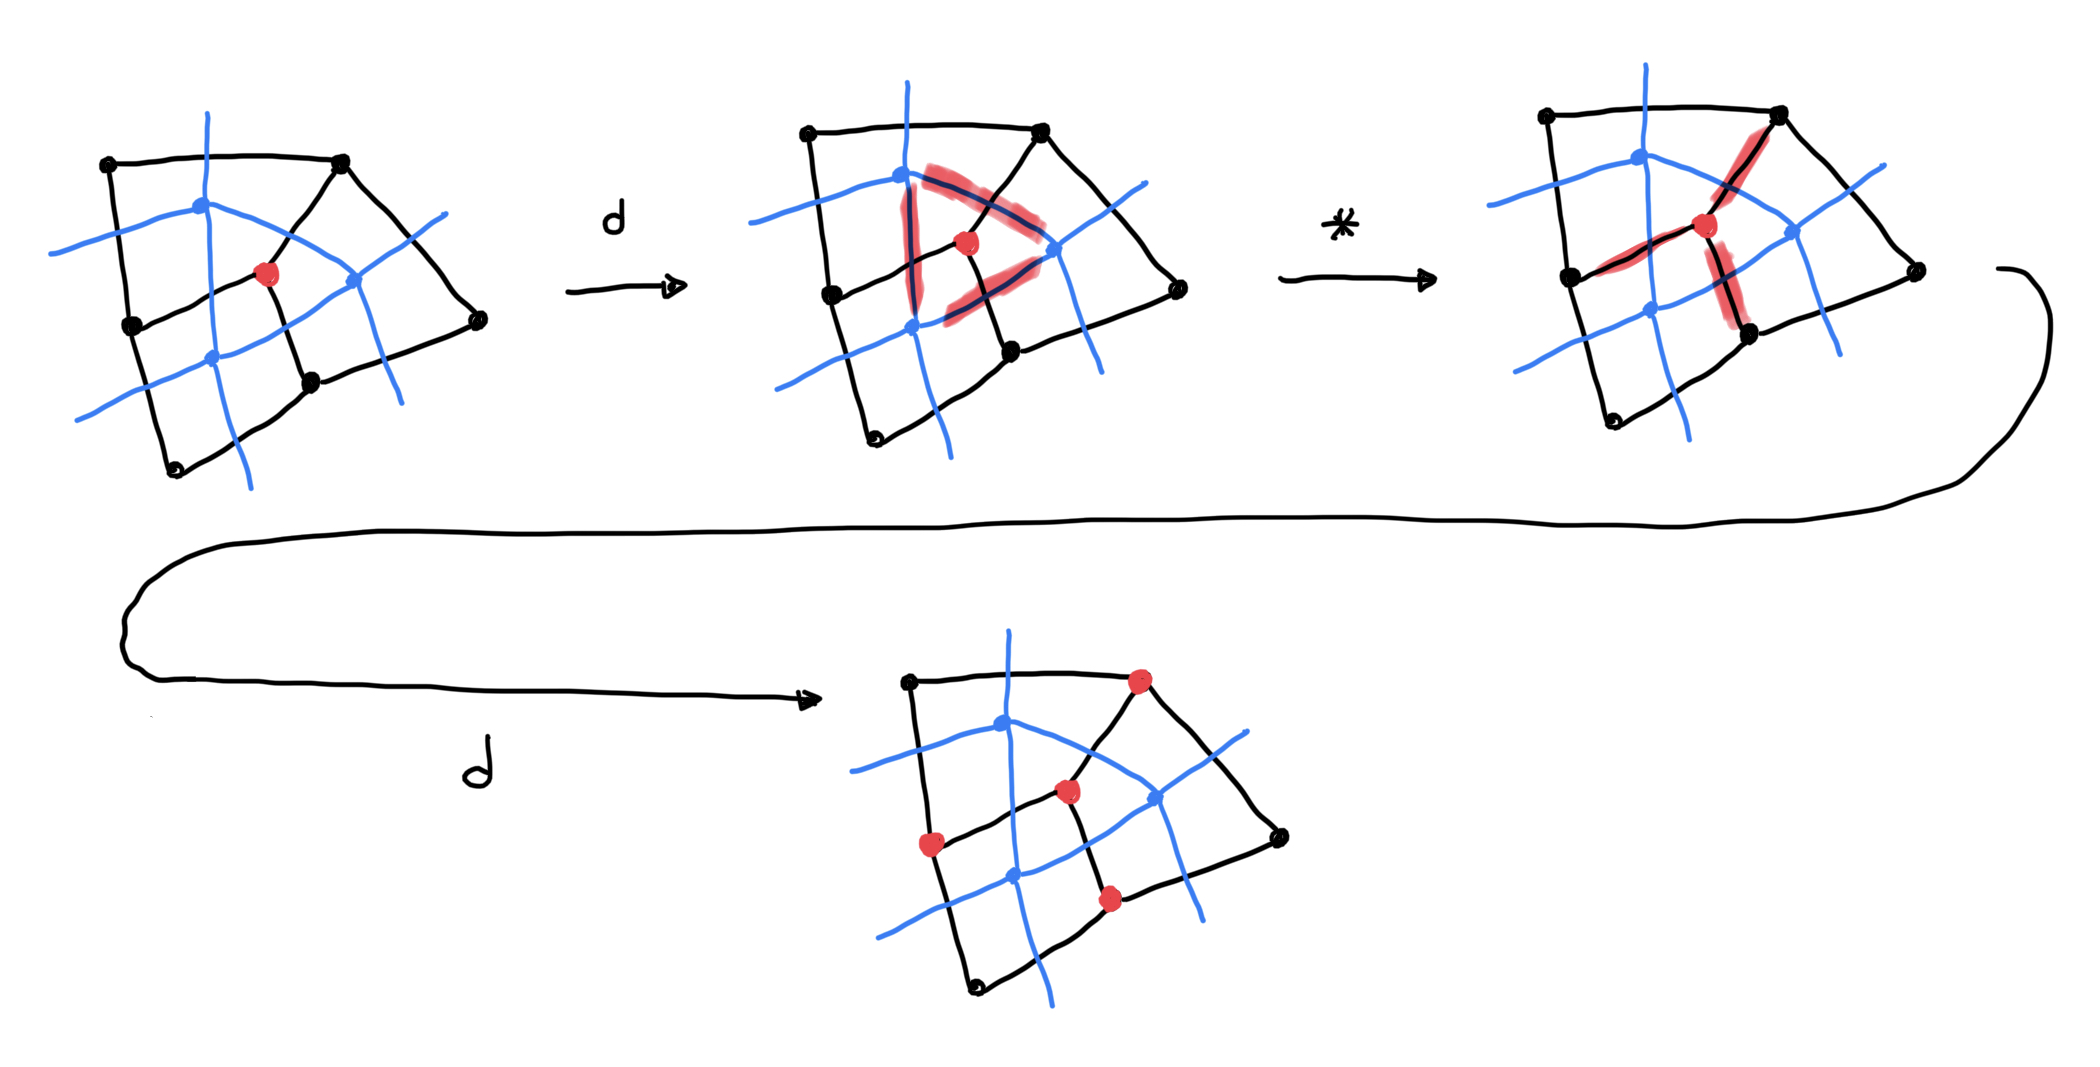
\includegraphics[width=\textwidth]{./assets/diag.jpeg}
  \end{center}

\section{Discrete Hodge decomposition}

\noindent To conclude this set of notes, we demonstrate that the Hodge decomposition, an important result in standard Hodge theory, holds
in the discrete case. First, let us make note of the fact that one can easily define an inner product on each of the spaces of $k$-cochains.
For functions, we simply use the naive inner product, summing over products evaluated at each vertex:
\begin{equation}
  \langle f, g \rangle \coloneqq \displaystyle\sum_{x \in \Lambda_{0}} f(x) \overline{g(x)}
\end{equation}
Similarly, for $2$-forms, we use the isomorphism between $C^2(\Lambda)$ and $C^0(\Lambda)$ to define $\langle \omega, \nu \rangle \coloneqq \langle * \omega, * \nu \rangle$.
Finally, for $1$-forms,
\begin{equation}
  \langle \alpha, \beta \rangle = \displaystyle\sum_{e \in \Lambda_1} \rho(e) \left( \displaystyle\int_{e} \alpha \right) \left( \displaystyle\int_{e} \overline{\beta} \right) 
\end{equation}
where, similar to the case for functions and $2$-forms, we are simply summing over products evaluated on all edges.

\begin{lemma}
  The operator $d^{\dagger} \coloneqq - * d *$ is, depending on the choice of $d$ and $*$, a map from $1$-forms to functions and $2$-forms to $1$-forms (it is the $0$-map on functions).
  In particular, $d^{\dagger}$ is the adjoint of the coboundary $d$ with respect to the inner products defined above.
\end{lemma}
\begin{proof}
  We can verify directly from definitions in each case. Both proof are similar, so we will only explicitly write out the case of $0$-forms/$1$-forms. In particular,
  \begin{align}
    \langle - * d * \alpha, g \rangle = -\displaystyle\sum_{x \in \Lambda_0} (* d *)(\alpha)(x) \overline{g(x)} &= -\displaystyle\sum_{x} \left( \displaystyle\int_{x^{*}} (d *)(\alpha) \right) \overline{g(x)} =
    -\displaystyle\sum_{x} \left( \displaystyle\int_{\partial x^{*}} * \alpha \right) \overline{g(x)} \\ &= \displaystyle\sum_{x \in \Lambda_0} \displaystyle\sum_{y \in n(x)} \rho(x, y) \left( \displaystyle\int_{(x, y)} \alpha \right) \overline{g(x)}.
  \end{align}
  From here, note that summing over each vertex in the double, then summing over all of its neighbours is equivalent to summing over the edges of $\Lambda$ twice, with each orientation included in the sum once. In particular,
  \begin{align}
    \displaystyle\sum_{x \in \Lambda_0} \displaystyle\sum_{y \in n(x)} \rho(x, y) \left( \displaystyle\int_{(x, y)} \alpha \right) \overline{g(x)} &= \displaystyle\sum_{(x, y) \in \Lambda_1} \rho(x, y) \left[  \left( \displaystyle\int_{(x, y)} \alpha \right) \overline{g(x)} + \left( \displaystyle\int_{(y, x)} \alpha \right) \overline{g(y)} \right]
    \\ & = \displaystyle\sum_{(x, y) \in \Lambda_1} \rho(x, y) \left( \displaystyle\int_{(x, y)} \alpha \right) \left( \overline{g(x)} - \overline{g(y)} \right)
    \\ & = \displaystyle\sum_{e \in \Lambda_1} \rho(e)  \left( \displaystyle\int_{(x, y)} \alpha \right) \left( \displaystyle\int_{(x, y)} \overline{dg} \right) = \langle \alpha, dg \rangle.
  \end{align}
  Thus, by definition, $- * d *$ is the adjoint of $d$, in this case.
\end{proof}

\noindent This result leads us finally to the discrete analogue of the \emph{Hodge decomposition}:

\hhrulefill

\begin{theorem}[Hodge decomposition]
  Let $\Sigma$ be a compact manifold, let $\Lambda$ be a discrete double on the surface. Then the space
  of $k$-forms $C^{k}(\Lambda)$ can be decomposed in an orthogonal direct sum as:
  \begin{equation}
    C^{k}(\Lambda) = \text{Im}(d) \oplus^{\perp} \text{Im}(d^{\dagger}) \oplus^{\perp} \text{Ker}(\Delta)
  \end{equation}
  In addition,
  \begin{equation}
    \text{Ker}(\Delta) = \text{Ker}(d) \cap \text{Ker}(d^{\dagger}).
  \end{equation}
 \end{theorem}

\hhrulefill
\newline

\noindent Before proceeding, let us make note of one more useful fact:

\begin{remark}
  In the case that $\Sigma$ is a compact surface, it is true that any double $\Lambda$ that is placed on $\Sigma$ must be \emph{finite} (this is due to the fact that the interiors of the faces of $\Lambda$ form
  an open cover for $\Sigma$, and there is a finitely-many-to-one pairing between edges and vertices, and faces). Therefore, the module formed by taking formal combinations of $k$-chains, $C_k(\Lambda)$ must too be finite dimensional.
  The dual space $C^{k}(\Lambda)$ is also finite dimensional. Thus, when discussing these modules, we are able to use all of the standard facts about finite dimensional vector spaces.
\end{remark}

\hhrulefill
\newline

\noindent We begin by demonstrating that $\text{Ker}(\Delta) = \text{Ker}(d) \cap \text{Ker}(d^{\dagger})$. Via the formula $\Delta = -d * d * - * d * d = -d d^{\dagger} - d^{\dagger} d$, it is clear that
$\text{Ker}(d) \cap \text{Ker}(d^{\dagger}) \subset \text{Ker}(\Delta)$. To prove the reverse inclusion, note that if $\Delta v = 0$, then $(d d^{\dagger} + d^{\dagger} d) v = 0$. Thus,
\begin{equation}
  \langle (d d^{\dagger} + d^{\dagger} d) v, v \rangle = 0 \Longrightarrow \langle d^{\dagger} v, d^{\dagger} v \rangle + \langle dv, dv \rangle = 0
\end{equation}
Since both of these inner products are necessarily non-negative, $dv = d^{\dagger} v = 0$, and the claim is proved. From here,
we can prove the first claim. In particular, since we are dealing with finite-dimensional vector spaces (see the remark above), we can always decompose into an orthogonal direct sum of a subspace
and its orthogonal complement. In particular,
\begin{equation}
  C^{k}(\Lambda) = \text{Im}(d) \oplus^{\perp} \text{Im}(d)^{\perp}
\end{equation}
Note then that
\begin{align}
  v \in \text{Im}(d)^{\perp} \Longleftrightarrow \langle v, d w \rangle = 0 \ \ \forall w \in C^{k - 1}(\Lambda) \Longleftrightarrow \langle d^{\dagger} v, w \rangle = 0 \ \ \forall w \in C^{k - 1}(\Lambda)
\end{align}
which is of course equivalent to $d^{\dagger} v = 0$, and $v \in \text{Ker}(d^{\dagger})$. Clearly, $(d^{\dagger})^2 = 0$. Therefore, $\text{Im}(d^{\dagger}) \subset \text{Ker}(d^{\dagger})$.
We again use the same strategy to write:
\begin{equation}
  \text{Ker}(d^{\dagger}) = \text{Im}(d^{\dagger}) \oplus^{\perp} \left( \text{Ker}(d^{\dagger}) \cap \text{Im}(d^{\dagger})^{\perp} \right)
\end{equation}
Once again, note that $\langle d^{\dagger} w, v \rangle = 0$ for all $w$ if and only if $dv = 0$, or in other words, $v \in \text{Ker}(d)$. We then conclude that
\begin{equation}
  \text{Im}(d^{\dagger}) \oplus^{\perp} \left( \text{Ker}(d^{\dagger}) \cap \text{Im}(d^{\dagger})^{\perp} \right) = \text{Im}(d^{\dagger}) \oplus^{\perp} \left( \text{Ker}(d^{\dagger}) \cap \text{Ker}(d) \right) = \text{Im}(d^{\dagger}) \oplus^{\perp} \text{Ker}(\Delta).
\end{equation}
The desired result follows immediately.

\end{document}
